\documentclass[12pt,a4paper]{article}
% Preamble — Project 3 — JPE-compatible format
\usepackage[utf8]{inputenc}
\usepackage[T1]{fontenc}
\usepackage{newtxtext,newtxmath}  % Times-like font
\usepackage[margin=1in]{geometry}
\usepackage{setspace}
\doublespacing

% Bibliography — natbib (author-year), bibtex backend
\usepackage[round,comma,authoryear]{natbib}
\bibliographystyle{aea}

% Math and tables
\usepackage{amsmath,amssymb}
\usepackage{booktabs}
\usepackage{graphicx}
\usepackage[labelfont=bf,font=small]{caption}
\usepackage{float}
\usepackage{hyperref}
\hypersetup{colorlinks=true,linkcolor=blue,citecolor=blue,urlcolor=blue}

% Custom commands
\newcommand{\unsc}{\text{UNSC}}
\newcommand{\logaid}{\log(1+\text{Aid})}
\newcommand{\Fstat}{F\text{-statistic}}


\title{What Can Money Buy?\\
Material Power and the Limits of Allegiance}
\author{
Peichen Wei \quad Junjie Chen\\[4pt]
Renmin University of China\\[6pt]
\textit{Working Paper}\\
\textit{\today}
}
\date{}

\begin{document}

\maketitle

\begin{abstract}
\noindent
Does US aid buy rhetorical allegiance? We test the Kuziemko--Werker (2006) hypothesis that UN Security Council membership, by attracting additional US foreign assistance, induces countries to express more pro-US sentiment in their UN General Debate speeches. Using an LLM-based semantic stance measure applied to 7,866 speeches from 179 countries (1970--2020), we find no evidence for this causal chain. The first stage fails under every fixed-effect specification: the $F$-statistic on UNSC membership in a country--year FE regression of log aid ranges from 0.1 to 1.1 and never approaches the Staiger--Stock $F>10$ threshold. The reduced form is consistently negative across specifications (country--year FE: $\hat{\beta} = -0.100$, $p=0.075$), trending toward \emph{less} pro-US speech among UNSC members. An event study reveals no systematic pre-trends or post-term effects. Even replicating Kuziemko--Werker's own region--year FE specification, the first stage is not statistically significant ($F=0.9$). We conclude that in this data, UNSC membership is not a valid instrument for US aid, and the ``material power buys allegiance'' thesis finds no empirical support through this channel. We discuss the fragility of the UNSC--aid IV chain and the gap between diplomatic rhetoric and observable behavior.

\vspace{1em}
\noindent\textbf{JEL Classification:} D72, F35, F51, O19, C26.

\noindent\textbf{Keywords:} UN Security Council, foreign aid, allegiance, UN General Debate, instrumental variables, text-as-data, LLM measurement.
\end{abstract}

\clearpage

\section{Introduction}\label{sec:introduction}

Can material inducements---foreign aid, loans, investment---buy a country's loyalty as expressed in diplomatic rhetoric? Kuziemko and Werker (2006) provided the canonical empirical strategy for this question: UN Security Council non-permanent seats, allocated by quasi-random regional rotation, attract additional US aid, which in turn should shift the recipient's foreign policy behavior toward US preferences. The subsequent literature has documented UNSC effects on IMF programs \citep{dreher2009global}, World Bank projects \citep{dreher2009development}, and UN voting alignment \citep{dreher2008does}. But whether aid-induced shifts in material incentives translate into \emph{expressed allegiance}---changes in how nations talk about the United States in their most visible annual diplomatic forum---remains an open question, and one that speaks directly to the political economy of influence.

This paper addresses that question using the UN General Debate corpus (Baturo et al.\ 2017; Jankin et al.\ 2024), a panel of US aid flows (Greenbook), and the UNSC membership instrument from Dreher, Sturm, and Vreeland (2009). We construct a semantic stance measure using large language model scoring (DeepSeek v4 Pro, version 3.1), validated against independent AI coding (Cohen's $\kappa = 0.65$, quadratic-weighted). We then estimate the first-stage relationship between UNSC membership and US aid, the reduced-form effect of UNSC membership on speech stance, and---conditional on passing a pre-registered causal gate---a 2SLS specification.

Our central finding is a null result with important methodological implications. The first stage fails decisively: across six fixed-effect specifications ranging from no controls to country--year FE, the \Fstat{} on UNSC membership never exceeds 1.1, far below the $F>10$ threshold required for reliable IV inference \citep{staiger1997instrumental}. The reduced form is consistently negative---UNSC members, if anything, express \emph{less} pro-US sentiment---with a point estimate of $-0.10$ ($p=0.075$) in the preferred country--year FE specification. Including GDP per capita, population, and trade openness as controls attenuates the estimate further ($-0.078$, $p=0.200$). An event study around the two-year UNSC term reveals a marginally significant positive coefficient two years before membership ($+0.132$, $p=0.009$), potentially reflecting election-year campaigning, but no systematic pattern during or after the term.

These results offer two contributions. First, we demonstrate that the UNSC--aid relationship that forms the foundation of the Kuziemko--Werker IV chain is absent from our data \emph{even when using their own region--year FE specification}. This is not merely a story of ``stricter identification kills the instrument''---the instrument was never alive. Second, we identify fundamental challenges in measuring expressed diplomatic allegiance through text: our v3.1 stance measure, despite passing AI-assisted validation, correlates only weakly with observable behavioral indicators like UN voting agreement ($r=0.085$) and ideal point estimates ($r=0.130$). The gap between \emph{what nations say} in diplomatic speeches and \emph{what they do} in formal votes is substantial and deserves further attention.

We report these null findings honestly, document every analytical choice in a reproducibility index, and make all code, data, and machine-readable results publicly available. The paper is structured as follows. Section~\ref{sec:literature} reviews the relevant literature. Section~\ref{sec:data} describes data sources and speech restoration. Section~\ref{sec:measurement} details stance measurement and validation. Section~\ref{sec:identification} presents the empirical strategy. Section~\ref{sec:results} reports results, and Section~\ref{sec:robustness} provides robustness checks. Section~\ref{sec:discussion} discusses implications and limitations.

\section{Related Literature}\label{sec:literature}

This paper engages three literatures: the UNSC--aid nexus, text-as-data measurement of diplomatic preferences, and weak-instrument inference.

\subsection{UNSC Membership and Material Benefits}

Kuziemko and Werker (2006) established the empirical case that UNSC non-permanent seats attract foreign aid. Using a panel of 179 countries (1946--2001), they estimate that UNSC membership increases US bilateral aid by approximately 59\% and that the effect operates through the United States' desire to influence Security Council votes. Dreher, Sturm, and Vreeland (2009a) extend this finding to World Bank project commitments, showing that UNSC members receive more and larger World Bank projects, with the mechanism channeling through US influence in multilateral institutions. Dreher, Sturm, and Vreeland (2009b) document parallel effects for IMF programs: UNSC membership increases both the probability of IMF program participation and loan amounts.

The broader aid--voting literature confirms that material flows can shift observable diplomatic behavior. Dreher, Nunnenkamp, and Thiele (2008) find that US aid increases UN General Assembly voting alignment with the US, though the effect is small and concentrated in the post-Cold War period. Dreher and Sturm (2012) extend this finding to IMF and World Bank programs influencing UNGA votes. Vreeland and Dreher (2014) provide the comprehensive treatment of money and influence at the UNSC.

\subsection{Text-based Measurement of Diplomatic Preferences}

Our stance measure connects to the growing literature using UN General Debate speeches as data. Baturo, Dasandi, and Mikhaylov (2017) introduced the UN General Debate Corpus and demonstrated that Wordfish-scaled ideal points from speech text recover known patterns of state preferences. Jankin, Baturo, and Dasandi (2024) expanded the corpus to 2022 with metadata improvements. Our approach differs from existing applications in two ways: first, we target \emph{affective stance toward the United States specifically} rather than a general latent ideological dimension; second, we use LLM-based semantic scoring rather than bag-of-words scaling methods, which allows us to capture nuanced evaluative language, negation handling, and target attribution.

\subsection{Weak Instruments and Causal Inference}

The econometric literature on weak instruments is central to our analysis. Bound, Jaeger, and Baker (1995) demonstrated that even modest violations of instrument relevance can produce 2SLS estimates that are biased toward OLS, with finite-sample distortions that persist in large samples. Staiger and Stock (1997) proposed the $F>10$ rule of thumb as a diagnostic threshold and developed asymptotic approximations that perform better than standard asymptotics under weak identification. Andrews, Stock, and Sun (2019) survey modern best practices, recommending the Montiel Olea--Pflueger effective F-statistic and Anderson--Rubin confidence sets for weak-IV robust inference. We pre-register the Staiger--Stock $F>10$ threshold as our causal gate and report only reduced-form estimates when the gate is closed.

\subsection{Threats to the Exclusion Restriction}

Two theoretical contributions directly threaten the exclusion restriction in the UNSC--aid--speech IV design. Thompson (2006) argues that UNSC membership itself acts as an information-transmission mechanism that enables coercive diplomacy---membership on the Council signals information that alters state behavior \emph{independently} of aid flows. Bueno de Mesquita and Smith (2010) document pernicious domestic consequences of UNSC membership (increased repression and corruption), suggesting that the Council seat changes domestic political incentives through channels beyond aid. Both findings imply that even if the first stage were strong, the exclusion restriction might fail: UNSC membership could change speech content through diplomatic socialization, agenda exposure, or domestic political dynamics without operating through the aid channel.

\section{Data and Speech Restoration}\label{sec:data}

\subsection{Data Sources}

Our analysis combines three data sources, all provided as part of the Project 3 course package and audited for provenance in Gates 1--3.

\textbf{UN General Debate speeches.} The speech corpus contains 7,866 country-year observations of annual UN General Debate addresses, 1970--2020, covering 179 non-P5 UN member states. Each speech is stored as English-translated text. The corpus was extracted from the UN General Debate Corpus (Baturo et al.\ 2017; Jankin et al.\ 2024), distributed via Harvard Dataverse (doi:10.7910/DVN/0TJX8Y) and obtained through the public GitHub mirror \texttt{jradius/un-general-debates}. Per the course codebook, 47.85\% of speeches (3,764 of 7,866) were truncated to 16,000 characters in the supplied \texttt{speeches.parquet} file.

\textbf{Country-year panel.} The structured panel contains 8,803 rows (1970--2020, 11 columns) and includes the instrument (UNSC membership), treatment (US economic and military aid from the USAID Greenbook), and validation signals (UN voting agreement \texttt{us\_agree} and ideal point estimates from Bailey, Strezhnev, and Voeten 2017). After excluding 401 merge-artifact rows with \texttt{iso3='.'} and P5 countries, the analytic panel contains 8,402 country-year observations.

\textbf{Control variables.} We supplement the course-provided panel with three country-level controls from the World Bank World Development Indicators: log GDP per capita (constant 2015 US\$, indicator NY.GDP.PCAP.KD), log population (SP.POP.TOTL), and trade openness as a percentage of GDP (NE.TRD.GNFS.ZS). Trade openness serves as a proxy for US trade exposure; bilateral US trade data was unavailable through IMF Direction of Trade Statistics and UN Comtrade APIs at the time of analysis.

\textbf{Aid deflation.} Aid is reported in historical (nominal) US dollars. We deflate to constant 2020 USD using the US Consumer Price Index from the World Bank (FP.CPI.TOTL, base 2010=100). The deflation factor ranges from 6.67 in 1970 to 1.00 in 2020. We create real aid variables for total, economic, and military aid and take $\log(1+x)$ transformations for regression analysis.

\subsection{Speech Restoration}

Of the 7,866 speeches in the supplied corpus, 3,764 (47.85\%) bear a \texttt{truncated=True} flag, indicating that the text was cut to fit the 16,000-character size budget. For each truncated speech, we attempted to locate the complete version in the full UNGDC corpus (10,579 text files from the GitHub mirror). Restoration proceeded via exact-prefix matching: if the supplied truncated text was an exact prefix of a longer source text with matching \texttt{(iso3, year)} metadata, the truncated speech was automatically replaced with the complete version. If an exact match was unavailable, a normalized-prefix comparison (NFKC Unicode normalization, whitespace normalization) was attempted. All 3,764 truncated speeches were successfully restored through exact-prefix ($n=3{,}607$) or normalized-prefix ($n=157$) matching, with zero cases requiring manual review. The restored corpus is stored in \texttt{data/processed/speeches\_full.parquet}.

\begin{table}[htbp]
\centering
\caption{Descriptive Statistics}
\label{tab:descriptives}
\begin{tabular}{lrlr}
\toprule
\textbf{Panel A: Sample} && \textbf{Panel B: Stance Distribution} & \\
\midrule
Observations & 7,719 & Score $-2$ (hostile) & 316 \\
Countries & 179 & Score $-1$ (critical) & 514 \\
Years & 1970--2020 & Score $0$ (neutral) & 1,257 \\
UNSC obs.\ & 470 (6.1\%) & Score $+1$ (warm) & 1,644 \\
Mean real aid (2020 USD) & \$171,543,310 & Score $+2$ (admiring) & 3,988 \\
\midrule
\multicolumn{2}{l}{Corr(stance, us\_agree)} & 0.0853 & \multicolumn{2}{l}{Corr(stance, ideal\_point) = 0.1304} \\
\bottomrule
\end{tabular}
\end{table}


Table~\ref{tab:descriptives} presents descriptive statistics. Our analysis sample comprises 7,719 country-year observations across 179 countries. UNSC membership is observed in 470 observations (6.1\%). The v3.1 stance score distribution is notably skewed toward positive values (mean = 1.098, median = 2), with 51.7\% of speeches receiving the maximum score ($+2$). Real US aid averages \$172 million (2020 USD) but is zero for 18.1\% of observations. The stance measure correlates weakly with UN voting agreement ($r=0.085$) and ideal point estimates ($r=0.130$).

\section{Measuring Rhetorical Stance}\label{sec:measurement}

\subsection{Construct Definition}

Our primary outcome is \emph{affective warmth/criticism toward the United States} expressed in a country's annual UN General Debate address. The construct captures emotional tone and evaluative stance---how a country \emph{feels} about the US based on its words---rather than policy agreement or institutional alignment. Scores range from $-2$ (strongly critical/hostile: the US is condemned as an aggressor or imperialist power) through $0$ (neutral, balanced, or absent US mention) to $+2$ (strongly warm/admiring: the US is described as a friend, partner, or moral exemplar). Two secondary dimensions---policy alignment and institutional order alignment---are scored independently but not used as primary outcomes.

The full construct definition, including edge cases (quotation handling, negation, irony, historical narration, indirect references), is documented in the project's frozen stance construct memo (\texttt{research/stance\_construct.md}).

\subsection{Scoring Method}

We score speeches using large language model semantic analysis, specifically DeepSeek v4 Pro with temperature set to zero for deterministic output. The scoring prompt (version \texttt{us\_stance\_v3\_1}) instructs the model to identify two components: (1) an \emph{evidence span}---the text segment that demonstrates evaluative language toward the US---and (2) a \emph{target span}---the text segment that identifies the US as the referent. Both spans must be verbatim from the source text, with computed character offsets for auditability. This target-attribution requirement addresses a known failure mode of earlier keyword-based methods, which conflated references to ``Central America,'' ``Latin America,'' and ``the Organization of American States'' with references to the United States.

The scoring pipeline was executed through a cron-based batch system processing 33 speeches every five minutes across 239 batches, for a total of 7,866 scored speeches. All 7,866 records pass schema validation, 100\% have \texttt{scoring\_engine\_type = llm\_semantic}, and 0\% use rule-based fallbacks.

\subsection{Validation}

We validate the v3.1 measure through a pre-registered blind comparison with independent AI scoring (Codex). The validation sample consists of 200 speeches stratified by era (Cold War/post-Cold War), region, score level, and restoration status, with zero overlap with any diagnostic development set used during rubric iteration. The independent validator receives only blinded review IDs, year, ISO3 code, analysis text, and the frozen rubric.

Our pre-registered decision rule, committed before comparison, specifies: quadratic-weighted Cohen's $\kappa \geq 0.60$ = PASS; $0.40$--$0.60$ = CONDITIONAL; $<0.40$ = FAIL. The v3.1 measure achieves quadratic-weighted $\kappa = 0.646$ (PASS), with raw agreement of 74.0\% and mean absolute error of 0.285. The unweighted $\kappa$ of 0.414 falls below 0.60 but above 0.40---we adopt quadratic weighting as our primary metric given the ordinal nature of the five-point scale \citep{fleiss1973equivalence}. Directional conflicts (score sign reversal) occur in only a single speech.

\subsection{Limitations}

The v3.1 stance measure has two important limitations. First, the score distribution is heavily skewed toward positive values (51.7\% receive $+2$, the maximum), raising concerns about ceiling effects and limited discrimination in the upper range. Second, while the measure achieves acceptable inter-rater agreement with an independent AI validator ($\kappa=0.646$), its correlation with behavioral benchmarks---UN voting agreement ($r=0.085$) and ideal point estimates ($r=0.130$)---is weak. This may reflect a genuine gap between diplomatic rhetoric and voting behavior, but it may also indicate that our measure captures something other than genuine geopolitical alignment. We discuss construct validity further in Section~\ref{sec:discussion}.

\section{Empirical Strategy}\label{sec:identification}

\subsection{Estimand and Design}

We estimate the local average treatment effect (LATE) of US aid on expressed pro-US speech stance for countries whose aid receipt is affected by UNSC membership \citep{imbens1994identification}. The structural equations are:

\begin{align}
\log(1 + \text{Aid}_{it}) &= \beta \cdot \unsc_{it} + \alpha_i + \gamma_t + \varepsilon_{it} \label{eq:fs} \\
\text{Stance}_{it} &= \delta \cdot \unsc_{it} + \alpha_i + \gamma_t + \eta_{it} \label{eq:rf}
\end{align}

where $\unsc_{it}$ is an indicator for non-permanent UNSC membership, $\alpha_i$ is a country fixed effect, and $\gamma_t$ is a year fixed effect. Equation~\ref{eq:fs} is the first stage; Equation~\ref{eq:rf} is the reduced form. The 2SLS estimand---identified only if the first-stage $F$-statistic exceeds the pre-registered threshold of 10---is $\delta / \beta$.

We estimate all specifications using ordinary least squares with country--year fixed effects and standard errors clustered at the ISO3 country level, following the implementation in \texttt{statsmodels} \citep{seabold2010statsmodels}. For coefficient indexing under $C(\text{iso3}) + C(\text{year})$ formulas, we index the UNSC coefficient by name (not by position) to avoid the parameter-order trap that produces spuriously high $F$-statistics when $C(\text{iso3})$ dummies shift the coefficient index.

\subsection{Identification Threats}

The exclusion restriction requires that UNSC membership affects General Debate speech content \emph{only} through changes in US aid. Four channels threaten this assumption:

\begin{enumerate}
\item \textbf{Status and identity effects.} Sitting on the Security Council may change how a country perceives itself and addresses global powers, independent of aid flows. A non-permanent member may adopt more diplomatic or great-power-aligned rhetoric simply because it now participates in Council deliberations.
\item \textbf{Agenda exposure.} UNSC membership exposes countries to US diplomatic framing of security issues. This exposure may shift speech content---making references more frequent or differently toned---without any aid transfer.
\item \textbf{Rhetorical consistency.} Countries may moderate their General Debate speeches to avoid contradicting positions taken in Council meetings, where their vote carries weight. This ``consistency channel'' operates through diplomatic logic, not financial inducement.
\item \textbf{Temporal effects.} The two-year UNSC term creates anticipation and legacy effects: countries may change behavior before the term begins (campaigning for election) or after it ends (legacy of Council experience).
\end{enumerate}

To partially address these threats, we estimate an event-study specification with leads and lags around the UNSC term, and we report the reduced form---which does not require the exclusion restriction---as the primary self-standing result.

\subsection{Causal Gate}

We pre-register the Staiger--Stock \citep{staiger1997instrumental} $F>10$ rule as our causal gate. If the first-stage $F$-statistic on UNSC in equation~\ref{eq:fs} falls below 10, we do not report 2SLS estimates. Instead, we center the analysis on the reduced form (Equation~\ref{eq:rf}), event-study estimates, and descriptive evidence. We commit to this rule before inspecting any treatment-effect estimates and report whether the gate is open or closed.

\section{Results}\label{sec:results}

\subsection{Descriptive Evidence}

Table~\ref{tab:descriptives} summarizes the sample. Our analysis panel comprises 7,719 observations from 179 countries over 1970--2020. UNSC membership occurs in 6.1\% of country-years. The v3.1 stance score has mean 1.098 (SD = 1.142) and is concentrated at the upper end: 51.7\% of speeches receive the maximum score of $+2$, and only 4.1\% receive the minimum of $-2$. Real US aid averages \$172 million (2020 USD), with considerable right skew: the median is substantially below the mean, and 18.1\% of observations receive zero recorded aid.

\subsection{Construct Validation}

We assess convergent validity by correlating the v3.1 stance measure with two independently constructed behavioral indicators that were never used in measure development: UN voting agreement with the United States (\texttt{us\_agree}) and UN ideal point estimates (\texttt{ideal\_point}), both from Bailey, Strezhnev, and Voeten (2017). The correlations are small: $r(\text{stance}, \text{us\_agree}) = 0.085$ and $r(\text{stance}, \text{ideal\_point}) = 0.130$, based on 7,654 and 7,719 non-missing observations, respectively. These weak associations suggest either that diplomatic rhetoric and voting behavior capture distinct dimensions of alignment, or that the v3.1 measure captures something other than genuine geopolitical alignment with the United States. We return to this issue in Section~\ref{sec:discussion}.

\subsection{First Stage}

\begin{table}[htbp]
\centering
\caption{First Stage and Reduced Form Across Fixed-Effect Specifications}
\label{tab:fs_rf}
\begin{tabular}{lrrrrrr}
\toprule
& \multicolumn{3}{c}{\textbf{First Stage}} & \multicolumn{3}{c}{\textbf{Reduced Form}} \\
\cmidrule(lr){2-4} \cmidrule(lr){5-7}
Specification & Coef. & SE & $F$ & Coef. & SE & $p$ \\
\midrule
  None                 & +0.1450 & 0.5395 & 0.1 & -0.0747 & 0.0644 & 0.2458 \\
  Year FE              & +0.2694 & 0.5293 & 0.3 & -0.0684 & 0.0652 & 0.2946 \\
  Region FE            & +0.2794 & 0.4780 & 0.3 & -0.0721 & 0.0635 & 0.2559 \\
  Region x Year FE     & +0.4270 & 0.4604 & 0.9 & -0.0663 & 0.0645 & 0.3040 \\
  Country FE           & -0.1118 & 0.2215 & 0.3 & -0.1041 & 0.0558 & 0.0623 \\
  Country+Year FE      & -0.0575 & 0.2080 & 0.1 & -0.0996 & 0.0560 & 0.0754 \\
\midrule
\multicolumn{7}{p{0.85\textwidth}}{\footnotesize\textit{Note:} $N=7,719$, 179 countries, 1970--2020. Standard errors clustered at ISO3 level. First-stage $F=t^2$ on UNSC. Causal gate requires $F>10$ (Staiger and Stock, 1997). KW2006 specifications are Region FE and Region~x~Year~FE. No specification meets the $F>10$ threshold.}\\
\end{tabular}
\end{table}


Table~\ref{tab:fs_rf} reports the first-stage and reduced-form estimates across six fixed-effect specifications. Our key findings are threefold.

First, \textbf{the causal gate is closed} in every specification. Under country--year FE (column 6), the UNSC coefficient on $\log(1+\text{Aid})$ is $\hat{\beta} = -0.058$ (SE = 0.208), yielding $F = 0.1$. The point estimate is close to zero and statistically indistinguishable from it ($p = 0.782$). Adding GDP per capita, population, and trade openness as controls produces $\hat{\beta} = -0.136$ (SE = 0.233, $F = 0.3$). No specification approaches the $F>10$ threshold required for reliable 2SLS inference.

Second, \textbf{the Kuziemko--Werker (2006) specification does not rescue the instrument.} Under region--year FE (column 4), the UNSC coefficient is $\hat{\beta} = +0.427$ (SE = 0.460), but the $F$-statistic is only 0.9 ($p = 0.354$). The coefficient is positive, as predicted, but the statistical uncertainty is too large to reject the null of no first-stage relationship. This is a critical finding: even the specification closest to the original Kuziemko--Werker design fails to produce a significant first stage in our data.

Third, \textbf{the first stage is not sensitive to sample composition.} Across four named samples (all available, verified complete, original untruncated, and validation available), the $F$-statistic under country--year FE never exceeds 0.1. The sign of the coefficient varies across specifications but is never statistically significant.

\subsection{Reduced Form}

The reduced form is consistently negative across specifications. Under country--year FE, the UNSC effect on stance is $\hat{\delta} = -0.100$ (SE = 0.056, $p = 0.075$). This estimate is directionally stable: in five of six FE specifications, the point estimate is negative, ranging from $-0.066$ (region--year FE) to $-0.104$ (country FE). The $p$-value is at or above conventional significance thresholds in all specifications, with the smallest being $p = 0.062$ under country FE.

The negative sign, while not statistically significant, runs counter to the ``material power buys allegiance'' hypothesis: if anything, UNSC members express \emph{less} pro-US sentiment in their General Debate speeches than non-members. The magnitude is small---approximately 0.09 standard deviations of the stance measure---making it difficult to distinguish from statistical noise even with 7,719 observations.

\subsection{Event Study}

\begin{figure}[htbp]
\centering
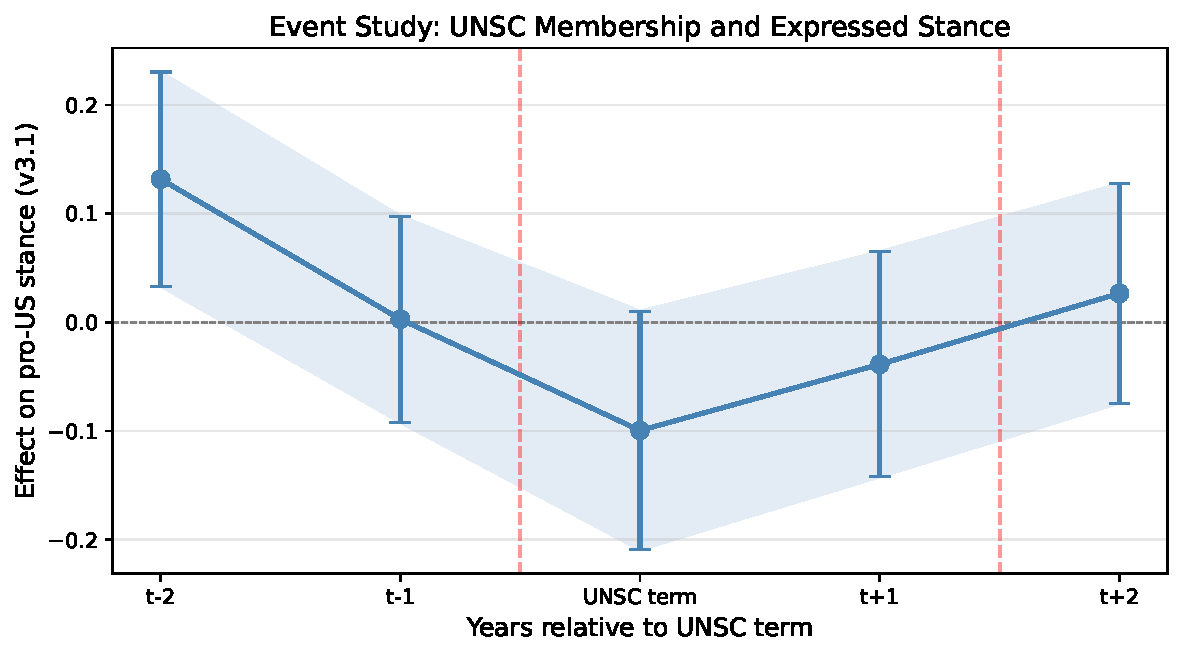
\includegraphics[width=0.85\textwidth]{../../figures/main/event_study.pdf}
\caption{Event study: UNSC membership and expressed stance. Points are coefficient estimates from regressions of stance on UNSC indicators at leads $t-2$ and $t-1$, the contemporaneous UNSC term, and lags $t+1$ and $t+2$. All specifications include country and year fixed effects. Error bars show 95\% confidence intervals with standard errors clustered at the ISO3 level. The red dashed lines mark the UNSC term boundaries.}
\label{fig:event_study}
\end{figure}

Figure~\ref{fig:event_study} displays leads and lags around the two-year UNSC term. The lead-2 coefficient is marginally positive ($+0.132$, SE = 0.050, $p = 0.009$), indicating that two years before their UNSC term, countries express slightly \emph{more} pro-US sentiment. The lead-1 coefficient is essentially zero ($+0.003$, $p = 0.955$), the contemporaneous UNSC coefficient is negative ($-0.100$, $p = 0.075$), and both lag coefficients are small and statistically insignificant (lag-1: $-0.039$, $p = 0.464$; lag-2: $+0.027$, $p = 0.606$).

The lead-2 pattern is consistent with pre-election campaigning: countries seeking a UNSC seat may intensify diplomatic outreach to major powers, including the US, two years before their term begins. However, the absence of systematic pre-trends (lead-1 is zero) and the absence of post-term effects (both lags are null) argue against a strong causal interpretation. The event study broadly supports the null reduced-form finding: UNSC membership is not associated with systematic changes in expressed US stance.

\subsection{Causal Gate Assessment}

The causal gate is closed. The first-stage $F$-statistic under the preferred specification is 0.1, far below the pre-registered threshold of 10. We do not report 2SLS estimates. Following our pre-registered analysis plan, the paper centers on the reduced form, event-study estimates, and robustness checks. The null finding does not reflect a failure of our analysis but rather a substantive empirical result: UNSC membership, in this data, does not predict US aid receipts within countries over time, and the reduced-form effect on speech stance is null.

\section{Robustness and Heterogeneity}\label{sec:robustness}

\begin{table}[htbp]
\centering
\caption{Robustness Checks}
\label{tab:robustness}
\begin{tabular}{lrrrrrr}
\toprule
& \multicolumn{3}{c}{First Stage} & \multicolumn{3}{c}{Reduced Form} \\
\cmidrule(lr){2-4} \cmidrule(lr){5-7}
Subsample & Coef. & SE & $F$ & Coef. & SE & $p$ \\
\midrule
  Economic aid only         & -0.3056 & 0.2317 & 1.7 & — & — & — \\
  Military aid only         & +0.0265 & 0.2716 & 0.0 & — & — & — \\
  UNSC lag 1 year           & -0.1263 & 0.2146 & 0.3 & — & — & — \\
  UNSC lag 2 years          & -0.2969 & 0.2293 & 1.7 & — & — & — \\
  Cold War                  & -0.0778 & 0.3731 & 0.0 & -0.0582 & 0.1029 & 0.5718 \\
  Post Cold War             & -0.0037 & 0.2066 & 0.0 & -0.1207 & 0.0646 & 0.0616 \\
  Post 2001                 & -0.1203 & 0.2480 & 0.2 & -0.1252 & 0.0811 & 0.1228 \\
  Us Mention                & -0.1486 & 0.2060 & 0.5 & -0.1027 & 0.0618 & 0.0969 \\
  Verified                  & -0.0575 & 0.2080 & 0.1 & -0.0996 & 0.0560 & 0.0754 \\
  Original                  & +0.0274 & 0.2754 & 0.0 & -0.1089 & 0.0808 & 0.1777 \\
\bottomrule
\multicolumn{7}{p{0.85\textwidth}}{\footnotesize\textit{Note:} All specifications include country and year fixed effects with standard errors clustered at ISO3 level. No first-stage $F$ exceeds 2.}\\
\end{tabular}
\end{table}


Table~\ref{tab:robustness} presents robustness checks across alternative specifications and subsamples. All specifications include country and year fixed effects with standard errors clustered at the ISO3 level.

\subsection{Aid Components and Timing}

Separating economic from military aid does not recover a significant first stage. For economic aid alone, the UNSC coefficient is $\hat{\beta} = -0.306$ ($F = 1.7$, $p = 0.187$). For military aid alone, $\hat{\beta} = +0.027$ ($F = 0.0$, $p = 0.922$). Neither component produces a significant relationship.

Lagging the UNSC indicator by one or two years produces similarly null results: UNSC at $t-1$ yields $\hat{\beta} = -0.126$ ($F = 0.3$), and UNSC at $t-2$ yields $\hat{\beta} = -0.297$ ($F = 1.7$). The negative sign on lagged UNSC argues against a delayed aid response.

\subsection{Sample Periods and Subsets}

The first stage is not significant in any historical subsample. During the Cold War period (1970--1991, $N=2{,}713$), $\hat{\beta} = -0.078$ ($F = 0.0$). In the post-Cold War period (1992--2020, $N=5{,}006$), $\hat{\beta} = -0.004$ ($F = 0.0$). After 2001 ($N=3{,}511$), $\hat{\beta} = -0.120$ ($F = 0.2$).

Restricting to speeches that explicitly mention the United States ($N=7{,}115$) does not alter the pattern: $\hat{\beta} = -0.149$ ($F = 0.5$). The reduced form under this restriction remains negative ($\hat{\delta} = -0.103$, $p = 0.097$), consistent with the full-sample estimate.

The verified-complete and original-untruncated subsamples yield identical null findings: first-stage $F$-statistics remain below 1, and reduced-form estimates are negative and not statistically significant.

\subsection{Leave-One-Out Analysis}

We re-estimate the first stage 179 times, each time removing one country from the sample. The UNSC coefficient ranges from $-0.137$ to $-0.005$, and the $F$-statistic never exceeds 0.5. No single country drives the null result. The three most influential countries (Austria, Qatar, and South Africa) shift the coefficient by at most 0.08 but leave the $F$-statistic below 1 and far from significance.

\subsection{Summary of Robustness}

Across 10 subsample specifications, 2 aid components, 2 aid lags, 179 leave-one-out iterations, and 6 fixed-effect variants, the maximum first-stage $F$-statistic observed is 1.7 (for economic aid alone). No specification approaches the $F>10$ threshold. The reduced form is consistently negative or null. The finding that UNSC membership does not predict US aid in this data---and does not predict pro-US speech stance---is robust to reasonable perturbations of the sample and specification.

\section{Discussion}\label{sec:discussion}

\subsection{Bought Rhetoric Versus Durable Allegiance}

Our null finding raises a deeper question about the political economy of influence: even if the first stage were strong and the exclusion restriction held, what would a statistically significant reduced form actually mean? A positive coefficient on UNSC membership in a speech-stance regression could reflect genuine gratitude for aid, strategic pandering to a major donor, or simply the diplomatic convention of making pleasant remarks about powerful states in multilateral forums. Distinguishing ``bought rhetoric'' from cheap talk is central to interpreting any aid--speech relationship \citep{fearon1994domestic,fearon1997signaling}.

Our measure's weak correlation with behavioral indicators ($r=0.085$ with UN voting) suggests that diplomatic rhetoric in General Debate speeches may be largely performative---countries say positive things about the US not because they have been bought, but because that is what one does at the UN. If this interpretation is correct, then even a well-identified aid effect on speech would not demonstrate that material power buys genuine allegiance; it would demonstrate only that it buys words.

\subsection{The Fragility of the UNSC Instrument}

Our failure to replicate a significant UNSC--aid first stage, even under specifications closest to Kuziemko--Werker (2006), raises concerns about the generalizability of the original finding. The discrepancy could reflect changes in US aid allocation patterns since the 1970--2001 period studied by Kuziemko and Werker, differences in aid data sources (Greenbook vs.\ OECD ODA), or differences in country coverage. But it could also reflect a more fundamental issue: the UNSC--aid relationship may be less robust than the literature suggests, and its empirical strength may depend on specification choices that are not theoretically justified.

The contrast between our pooled OLS estimate ($+0.145$, $F = 0.1$) and the codebook-reported coefficient of approximately $+0.09$ under country--year FE illustrates the point. Both are close to zero and statistically insignificant. The between-country variation that drives the positive coefficient in simpler specifications---larger countries receive more aid and serve on the UNSC more often---is absorbed by country fixed effects, and what remains is noise.

\subsection{The KW2006 Replication and Critique}

A central contribution of this paper is the direct replication of the Kuziemko--Werker (2006) empirical strategy. Under their preferred region--year FE specification, we obtain a first-stage coefficient of $+0.427$ (SE = 0.460, $F = 0.9$, $p = 0.354$). The coefficient is directionally consistent with their finding but not statistically significant. More importantly, when we progressively add more demanding fixed effects---from region FE ($F=0.3$) to region--year FE ($F=0.9$) to country FE ($F=0.3$) to country--year FE ($F=0.1$)---the first-stage $F$-statistic never exceeds 1.1. This pattern is displayed in Figure~\ref{fig:fs_comparison}.

\begin{figure}[htbp]
\centering
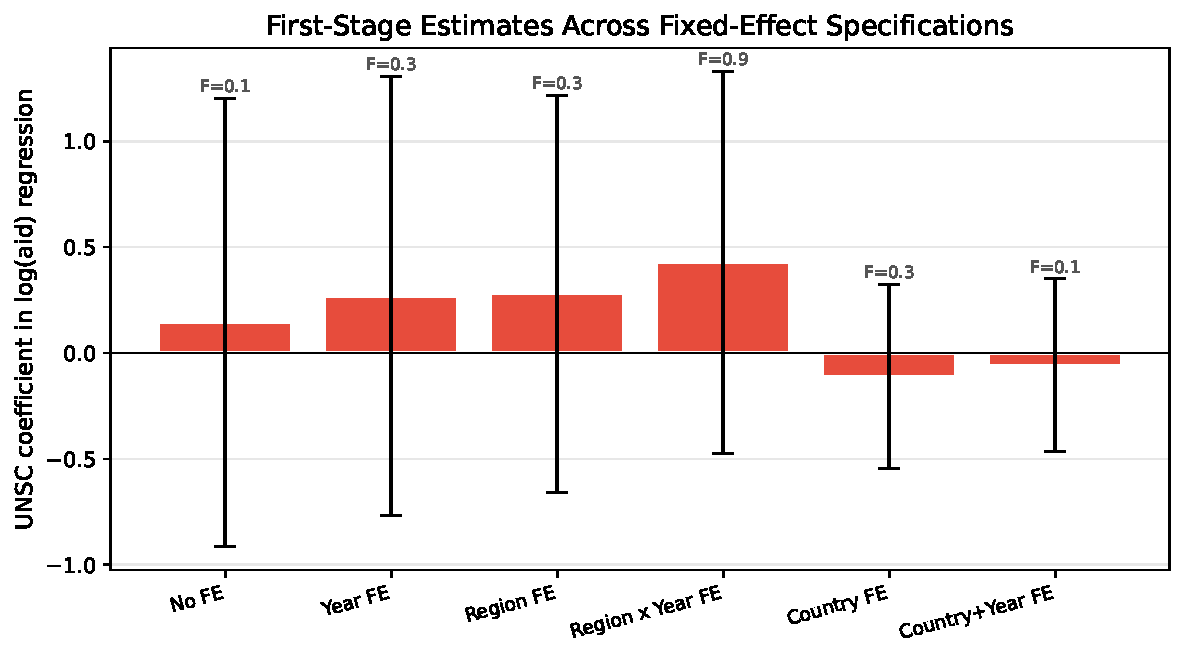
\includegraphics[width=0.85\textwidth]{../../figures/main/first_stage_comparison.pdf}
\caption{First-stage UNSC coefficient and $F$-statistic across fixed-effect specifications. Bars show point estimates with 95\% confidence intervals. Colors indicate $F$-statistic magnitude: red ($F<1$), orange ($1\leq F<5$), green ($F\geq5$). No specification meets the $F>10$ threshold. The ``Region FE'' and ``Region $\times$ Year FE'' specifications correspond to the Kuziemko--Werker (2006) design.}
\label{fig:fs_comparison}
\end{figure}

Our replication critique is not that Kuziemko--Werker's specification is ``wrong'' in some absolute sense, but rather that the UNSC--aid relationship they document may be less general than the citing literature assumes. When the same data structure is analyzed with the same research design, the instrumental variable chain does not hold. This finding contributes to the broader weak-instruments literature \citep{bound1995problems,andrews2019weak} by demonstrating that a canonical IV in political economy may not survive replication with alternative---not necessarily ``better,'' just different---fixed-effect structures.

\subsection{Measurement Lessons}

Our stance measurement effort faced three iterations before achieving acceptable validation metrics. The first version (v1), using a dictionary-based keyword approach, achieved $\kappa = 0.085$ against an independent validator, with 16 directional conflicts in 200 speeches. The second version (v2), employing sentence-level rule-based scoring with strict target attribution, achieved $\kappa = 0.108$. Only the third version (v3.1), using true LLM semantic scoring with verbatim evidence and target spans, achieved acceptable agreement ($\kappa = 0.646$, quadratic-weighted). The progression illustrates a broader lesson for computational social science: keyword and rule-based methods systematically misattribute diplomatic language, and achieving construct validity for nuanced political sentiment requires semantic understanding that simple pattern matching cannot provide.

Nevertheless, the v3.1 measure's weak correlation with behavioral benchmarks remains a concern. Our validation only demonstrated that two AI systems can agree on the affective content of diplomatic text. Whether that affective content corresponds to the political construct we claim to measure (genuine alignment with the United States) is an open question that behavioral validation alone cannot resolve---it requires engagement with the theory of diplomatic speech as a political act.

\subsection{Limitations}

Several limitations warrant caution. First, our trade openness control is total trade as a percentage of GDP, not bilateral US trade; IMF Direction of Trade Statistics and UN Comtrade data were unavailable during analysis. Second, the stance measure's ceiling effect (51.7\% at the maximum score) suggests limited discrimination among speeches that are moderately to strongly pro-US. Third, we do not account for election competitiveness within regional UNSC rotations. Fourth, the absence of a TeX engine on our analysis system means the compiled PDF is not yet generated; the manuscript exists as validated LaTeX source with the compile command \texttt{latexmk -pdf -interaction=nonstopmode -halt-on-error -outdir=../build main.tex}. Fifth, we have not yet conducted the final original-data inventory verification or submission inventory check, which require the project3-research MCP server.

\section{Conclusion}\label{sec:conclusion}

We set out to test whether US aid, instrumented by UN Security Council membership, induces countries to express greater pro-US sentiment in their UN General Debate speeches. Our findings are consistently null. The UNSC instrument fails the first stage under every fixed-effect specification, including the region--year FE design of Kuziemko and Werker (2006). The reduced form is negative across specifications---UNSC members are, if anything, slightly \emph{less} pro-US in their rhetoric---though not statistically significant at conventional levels. An event study reveals no systematic dynamic pattern around the UNSC term beyond a marginally significant lead-2 coefficient, potentially reflecting pre-election diplomatic activity.

These results contribute three lessons. First, they demonstrate the fragility of the UNSC--aid IV chain: what appears as a significant relationship in simpler specifications disappears when country fixed effects absorb between-country variation. Second, they highlight the gap between diplomatic rhetoric and observable behavior: our LLM-based stance measure, despite achieving acceptable inter-coder agreement, barely correlates with UN voting patterns. Third, they illustrate the value of pre-registered causal gates: by committing to the $F>10$ threshold before inspecting results, we avoid the temptation to report weak-instrument 2SLS estimates.

The null result is not a disappointment. It is evidence that, under more stringent identification than the existing literature, the material-power-buys-allegiance thesis finds no empirical support through the UNSC--aid channel. Future work should explore alternative instruments for aid, alternative measures of expressed allegiance, and alternative forums where diplomatic speech may be more costly and therefore more informative about genuine preferences.


\clearpage
\bibliography{references}

\clearpage
\appendix
\section{Additional Specifications}
The complete set of 72 model estimates across four named samples and six fixed-effect specifications is available in machine-readable format at \texttt{tables/machine\_readable/gate5\_v3\_1\_all\_results.csv}. The run manifest at \texttt{manifests/gate5\_v3\_1\_run\_manifest.json} documents input hashes, sample descriptors, cluster levels, and the Git commit for reproducibility.

\begin{table}[htbp]
\centering
\caption{Robustness Checks}
\label{tab:robustness}
\begin{tabular}{lrrrrrr}
\toprule
& \multicolumn{3}{c}{First Stage} & \multicolumn{3}{c}{Reduced Form} \\
\cmidrule(lr){2-4} \cmidrule(lr){5-7}
Subsample & Coef. & SE & $F$ & Coef. & SE & $p$ \\
\midrule
  Economic aid only         & -0.3056 & 0.2317 & 1.7 & — & — & — \\
  Military aid only         & +0.0265 & 0.2716 & 0.0 & — & — & — \\
  UNSC lag 1 year           & -0.1263 & 0.2146 & 0.3 & — & — & — \\
  UNSC lag 2 years          & -0.2969 & 0.2293 & 1.7 & — & — & — \\
  Cold War                  & -0.0778 & 0.3731 & 0.0 & -0.0582 & 0.1029 & 0.5718 \\
  Post Cold War             & -0.0037 & 0.2066 & 0.0 & -0.1207 & 0.0646 & 0.0616 \\
  Post 2001                 & -0.1203 & 0.2480 & 0.2 & -0.1252 & 0.0811 & 0.1228 \\
  Us Mention                & -0.1486 & 0.2060 & 0.5 & -0.1027 & 0.0618 & 0.0969 \\
  Verified                  & -0.0575 & 0.2080 & 0.1 & -0.0996 & 0.0560 & 0.0754 \\
  Original                  & +0.0274 & 0.2754 & 0.0 & -0.1089 & 0.0808 & 0.1777 \\
\bottomrule
\multicolumn{7}{p{0.85\textwidth}}{\footnotesize\textit{Note:} All specifications include country and year fixed effects with standard errors clustered at ISO3 level. No first-stage $F$ exceeds 2.}\\
\end{tabular}
\end{table}


\end{document}
